
\section{Proposed Method}

In domain generalization for multi-label ocular disease recognition, model performance is mainly affected by three factors. First, multiple diseases may coexist in the same fundus image. If the model cannot effectively capture relevance among disease labels and between labels and disease-related features, false positives and false negatives may occur, degrading multi-label recognition performance. Second, distribution shifts commonly arise between the source domain and target domain. If the learned features contain substantial source-domain-specific noise, the transferability of disease-related features is weakened, resulting in poorer domain generalization performance. In addition, medical data are privacy-sensitive, and the gradients or parameters produced during training may introduce privacy leakage risk, requiring a privacy-preserving mechanism to be incorporated into the training process. However, privacy-preserving mechanisms usually affect model optimization through additional training constraints, so the balance between privacy preservation and model performance must be considered.

To address these issues, this study does not treat multi-disease co-occurrence and domain shift as separate problems. Instead, they are jointly modeled within a single-domain generalization framework for multi-label ocular disease recognition. As shown in \hyperref[fig:method-framework]{Fig.~\ref*{fig:method-framework}}, the proposed interpretable single-domain generalization framework consists of two main parts: Part 1, Dual-Branch Guided Domain-Invariant Feature Extraction (DFE), and Part 2, Adaptive Label-Feature Relevance Construction (ARC). Part 1 uses CAM guidance together with a \revision{dual-branch feature filtering mechanism} to extract more stable domain-invariant features from a single source domain, thereby reducing the influence of distribution shift between the source domain and unseen domains. CAM also visualizes model-attended regions and enhances interpretability. Based on the domain-invariant features produced by Part 1, Part 2 uses Transformer attention mechanisms to model label-label relevance and label-feature relevance, reducing false positives and false negatives in multi-label recognition. \revision{DFE and ARC are connected through feature filtering and label-representation consistency. DFE first selects feature components with small normalized differences between the two views as inputs to ARC. ARC then extracts a representation for each disease label and constrains the corresponding representations to remain close across the two views. The classification and consistency objectives jointly guide feature learning, applying the stability requirement under appearance perturbations to the representations associated with disease labels.} \revision{The framework adopts single-source domain generalization, restricting training updates to the accessible source domain and reducing the need to access target-domain training data or pool raw data across institutions. Building on this setting, AdaGDP is applied to the training updates of the joint DFE and ARC model to further protect source-domain training information. Its noise schedule aims to preserve recognition performance as much as possible.} Overall, the proposed method constructs a Privacy-Preserving Interpretable Single-Domain Generalization framework for multi-label ocular disease recognition. The implementation details of each module are described in the following three subsections.

\begin{figure}
\centering
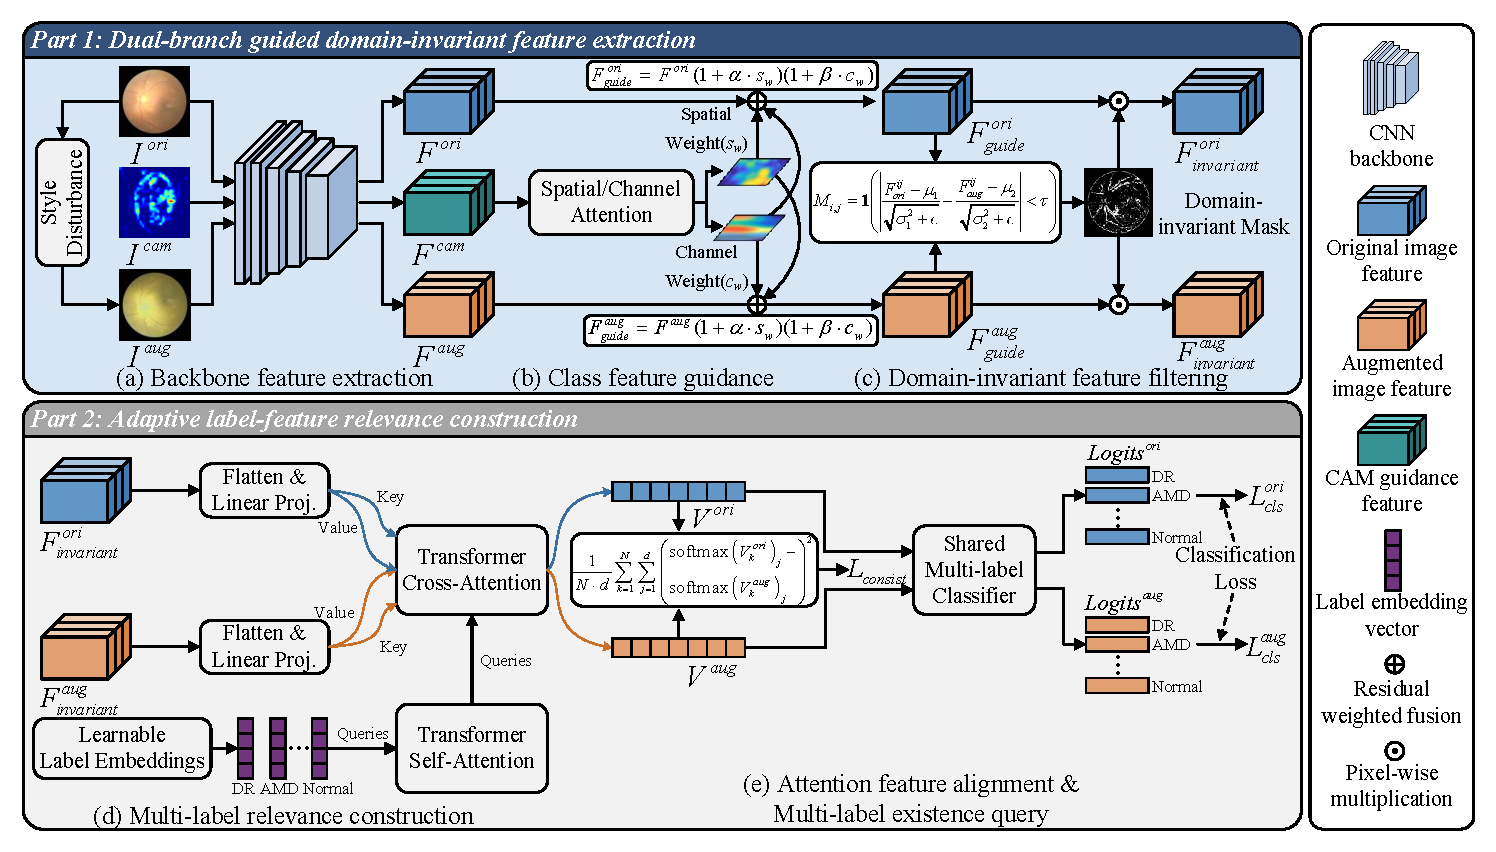
\includegraphics[width=0.96\textwidth]{images/media/image2_padded.pdf}
\caption{Overview of the proposed interpretable single-domain generalization framework. Part 1 is Dual-Branch Guided Domain-Invariant Feature Extraction (DFE), consisting of (a)--(c): (a) original source-domain images and augmented source-domain images are first fed into the backbone to extract dual-branch features; (b) CAM is used to generate model-attended region guidance, which enhances disease-related regions and suppresses background noise; and (c) a \protect\revision{dual-branch feature filtering mechanism} \protect\revision{compares normalized feature differences between the two views to retain components that are relatively stable under the selected appearance perturbations.} Part 2 is Adaptive Label-Feature Relevance Construction (ARC), consisting of (d)--(e): (d) Transformer self-attention is used to model label-label relevance, and cross-attention is then used to establish label-feature relevance; (e) attention consistency constraints improve the stability of attention features, thereby reducing false positives and false negatives in multi-label recognition.}
\label{fig:method-framework}
\end{figure}

\subsection{Dual-Branch Guided Domain-Invariant Feature Extraction}

\revision{Considering that multi-institutional data in medical scenarios are often difficult to centralize or use synchronously, this study adopts a single-domain generalization setting. DFE aims to learn disease-discriminative representations from a single source domain, with cross-domain stability as its learning objective.} Inspired by contrastive learning, original source-domain images are transformed into augmented source-domain images through augmentation techniques such as style disturbance to simulate possible distribution shifts in unseen domains. Specifically, \(I^{ori}\) denotes original source-domain images, and \(I^{aug}\) denotes augmented source-domain images generated by style disturbance, such as MixStyle or random adjustment of brightness, contrast, and saturation. \revision{This augmentation is designed to simulate appearance variations associated with imaging devices and illumination conditions while preserving disease-related semantic content.}

First, as shown in \hyperref[fig:method-framework]{Fig.~\ref*{fig:method-framework}.a}, both \(I^{ori}\) and \(I^{aug}\) are fed into the backbone network to extract features \(F^{ori}\) and \(F^{aug}\). Let \(F^{ori} \in \mathbb{R}^{C \times H \times W}\) and \(F^{aug} \in \mathbb{R}^{C \times H \times W}\), where \(C\), \(H\), and \(W\) denote the number of channels, height, and width of the final feature map of the backbone network, respectively. ResNet50 \cite{_RefResNet2016} is selected as the backbone because it performs well in image recognition tasks and offers good feature extraction capability and computational efficiency. However, relying only on contrastive constraints between original and augmented source-domain images remains limited. The model may still learn domain-specific noise such as background textures, illumination variations, or image-edge artifacts, which can affect multi-label ocular disease recognition on unseen domains.

\revision{To this end, the framework incorporates the class feature guidance module} shown in \hyperref[fig:method-framework]{Fig.~\ref*{fig:method-framework}.b} to improve the disease relevance and interpretability of features. A CAM guidance map is generated on the training set in advance using the baseline model, namely ResNet50 with BCE loss. The CAM guidance map highlights the regions attended by the model for different diseases; for example, Diabetic Retinopathy (DR) mainly corresponds to vascular regions, whereas Age-Related Macular Degeneration (AMD) mainly corresponds to the macular region. For a target class \(c\), it is calculated as follows:

\begin{equation}\label{eq:cam}
I^{cam,c} = \operatorname{ReLU}\left(\sum_{k = 1}^{C}\omega_{k}^{c} \cdot A_{k}\right),
\end{equation}

Here, \(A_{k}\) is the activation map of the \(k\)-th channel in the last convolutional layer of the backbone network, and \(\omega_{k}^{c}\) is the importance weight of the \(k\)-th channel for target class \(c\). It is obtained by global average pooling the gradient of the class score \(y^{c}\) with respect to the channel activation map:

\begin{equation}\label{eq:cam-weight}
\omega_{k}^{c} = \frac{1}{Z}\sum_i\sum_j \frac{\partial y^{c}}{\partial A_{ij}^{k}},
\end{equation}

where \(Z\) denotes the number of spatial locations in the feature map. This Grad-CAM-based formula produces a class-specific spatial attention heatmap rather than a raw fundus image. In practice, one or more \(I^{cam,c}\) maps are generated according to the positive labels or predicted classes of an image, and they are normalized and resized to form the CAM guidance map \(I^{cam}\). The resulting \(I^{cam}\) is then fed into the backbone network to obtain \(F^{cam} \in \mathbb{R}^{C \times H \times W}\). Spatial attention weights \(s_{w}\) and channel attention weights \(c_{w}\) are then computed from \(F^{cam}\) through spatial and channel attention modules, respectively. Both attention modules are convolutional sequential networks containing \(1 \times 1\) convolution, ReLU activation, and a Sigmoid function for adaptive weight generation. The spatial attention module additionally combines average and max pooling to capture local context, generating a pixel-level weight map that adaptively enhances the saliency of lesion regions, such as vessels or the macula, while suppressing background noise. The channel attention module uses adaptive average pooling to compress spatial dimensions and obtain global statistics, then learns channel dependencies to enhance disease-texture-sensitive channels and suppress noisy channels. The two weights are applied to \(F^{ori}\) and \(F^{aug}\) to obtain CAM-guided features \(F_{guide}^{ori}\) and \(F_{guide}^{aug}\). A residual connection is used in the weighting operation to avoid damaging original information through excessive guidance:

\begin{align}
F_{guide}^{ori} &= F^{ori}(1 + \alpha{\cdot s}_{w})(1 + {\beta \cdot c}_{w}), \label{eq:guide-feature-ori} \\
F_{guide}^{aug} &= F^{aug}(1 + \alpha{\cdot s}_{w})(1 + {\beta \cdot c}_{w}), \label{eq:guide-feature-aug}
\end{align}

Here, \(\alpha\) and \(\beta\) are hyperparameters that control the enhancement strengths of \(s_{w}\) and \(c_{w}\), respectively. Residual weighting allows CAM guidance to highlight disease-related regions while retaining the original feature representation, reducing the model's reliance on domain-specific noise such as illumination and background textures. \revision{The resulting guided representations serve as inputs to the subsequent dual-branch feature filtering.} Meanwhile, visualizing model-attended regions through CAM enhances model interpretability and helps clinicians understand the basis of prediction, for example by overlaying CAM to inspect whether the model focuses on lesion regions.

\revision{Next, the framework applies a dual-branch feature filtering mechanism}, as shown in \hyperref[fig:method-framework]{Fig.~\ref*{fig:method-framework}.c}. \revision{The original and augmented images provide two views of the same source-domain sample under different appearance conditions. After instance normalization of the guided features from both views, their differences are compared element by element, and components with small differences are retained to reduce the influence of features that are sensitive to the selected appearance perturbations on subsequent label-representation learning.} The mask matrix \(M \in \mathbb{R}^{C \times H \times W}\) is calculated from the normalized distance:

\begin{equation}\label{eq:mask}
M_{ij} =
\left\{
\begin{array}{ll}
1, & \text{if } \left| \dfrac{F_{guide}^{ori,ij} - \mu_{1}}{\sqrt{\sigma_{1}^{2} + \epsilon}} - \dfrac{F_{guide}^{aug,ij} - \mu_{2}}{\sqrt{\sigma_{2}^{2} + \epsilon}} \right| \leq \tau, \\
0, & \text{otherwise.}
\end{array}
\right.
\end{equation}

Here, \(\mu_{1},\sigma_{1}\) and \(\mu_{2},\sigma_{2}\) are the means and variances of the two guided features, respectively, \(\epsilon = 10^{-5}\) is a stability constant, and \(i,j\) denote feature map positions. Components satisfying the threshold \(\tau\) are assigned 1, while the remaining components are assigned 0. \revision{The threshold $\tau$ controls the feature differences allowed between the two views. For a fixed pair of feature maps, a smaller threshold imposes stricter filtering, whereas a larger threshold retains more features. It therefore controls the trade-off between information retention and perturbation suppression. Overly strict filtering may remove useful information that is sensitive to augmentation, whereas a more permissive threshold may retain more components affected by appearance variations.} The mask matrix is then applied to \(F_{guide}^{ori}\) and \(F_{guide}^{aug}\) \revision{to retain components with small normalized differences between the two views:}

\begin{equation}\label{eq:invariant-feature}
F_{invariant}^{ori} = F_{guide}^{ori} \odot M,F_{invariant}^{aug} = F_{guide}^{aug} \odot M,
\end{equation}

Here, \(\odot\) denotes pixel-wise element-wise multiplication. \revision{The filtered features from both branches are passed to the subsequent label-feature relevance module, allowing disease-label queries to operate on feature components that are relatively consistent across the two views. This mechanism is designed on the premise that augmentation preserves disease information shared by both views. When augmentation alters subtle lesion cues, the normalized feature differences between the views may increase beyond the threshold, causing features useful for disease discrimination to be filtered out. When background interference remains stable across both views, its feature differences may still satisfy the retention criterion, allowing it to pass through the mask. Its operation should therefore be understood in relation to the augmentation strategy and the quality of CAM guidance.}

\subsection{Adaptive Label-Feature Relevance Construction}

\revision{Using the features filtered by DFE,} the model further handles the multi-label relevance problem caused by ocular disease co-occurrence. To this end, Transformer attention mechanisms are embedded to construct adaptive relevance at the label and feature levels for multi-label prediction. As shown in \hyperref[fig:method-framework]{Fig.~\ref*{fig:method-framework}.d} and \hyperref[fig:method-framework]{Fig.~\ref*{fig:method-framework}.e}, this module includes multi-label relevance construction and attention feature alignment.

First, the eight labels in the ODIR dataset, such as normal, DR, and AMD, are modeled as learnable vectors \(L = \lbrack L_{1},\ldots,L_{8}\rbrack \in \mathbb{R}^{8 \times d}\), where \(d = 512\) is the embedding dimension. These vectors are initialized from a random Gaussian distribution and optimized during training to characterize potential relevance among different disease labels. The label vectors are fed into the Transformer self-attention mechanism to model label relevance:

\begin{equation}\label{eq:self-attention}
V_{self} = \operatorname{softmax}\left(\frac{QK^{T}}{\sqrt{d_{k}}}\right)V,
\end{equation}

Here, \(Q = LW_{Q},K = LW_{K},V = LW_{V}\), where \(W_{Q},W_{K},W_{V}\) are learnable projection matrices and \(d_{k} = d/heads\) for multi-head attention with \(heads=8\). The self-attention output \(V_{self}\) captures label relevance, enabling different disease labels to interact dynamically according to co-occurrence patterns and visual evidence in the training data.

\revision{Next, a cross-attention mechanism is used to combine labels with the features filtered by DFE.} Since Transformer requires sequential input, \(F_{invariant}^{ori}\) and \(F_{invariant}^{aug}\) output by Part 1 are first flattened and used as Key and Value, while the label vector \(V_{self}\) is used as Query for cross-attention calculation:

\begin{equation}\label{eq:cross-attention}
V_{cross}^{ori} = \operatorname{softmax}\left(\frac{V_{self}W_{Q}(F_{invariant}^{ori}W_{K})^{T}}{\sqrt{d_{k}}}\right)(F_{invariant}^{ori}W_{V}),
\end{equation}

\(V_{cross}^{aug}\) is calculated in the same way. Through cross-attention weighting, labels are matched with corresponding disease features to form attention vectors \(V \in \mathbb{R}^{8 \times d}\), so that each label vector obtains a higher response on disease-related regions. In this process, each label vector is not matched with image features independently; instead, it queries image features based on the label relevance modeled by self-attention. The model can therefore focus on local lesion features corresponding to each disease while also using disease co-occurrence dependencies to support the prediction of other relevant labels, thereby reducing false positives and false negatives in multi-label recognition.

\revision{Provided that augmentation preserves disease semantics, the original image and its augmented view share the same disease labels. To encourage the representations associated with each disease label to remain consistent under appearance perturbations, a consistency constraint is imposed on the corresponding label representations after Softmax normalization in the two branches. This constraint complements the preceding mask: the mask filters the input features, whereas the consistency loss constrains the outputs of the two branches at the level of label-associated representations. The loss is calculated using mean squared error (MSE):}

\begin{equation}\label{eq:consistency-loss}
L_{consist} = \frac{1}{N \cdot d}\sum_{k = 1}^{N}\sum_{j = 1}^{d}
\left(
\operatorname{softmax}\left( V_{k}^{ori} \right)_{j}
-
\operatorname{softmax}\left( V_{k}^{aug} \right)_{j}
\right)^{2},
\end{equation}

Here, \(N = 8\) is the number of labels and \(d = 512\) is the embedding dimension. Softmax normalizes attention vectors into comparable distribution forms. The attention consistency loss improves model stability under domain shift by minimizing differences between normalized attention features of the two branches.

Finally, the attention vectors are fed into the multi-label classifier. LayerNorm and Dropout are first applied to the class query features for lightweight feature enhancement, normalization, and regularization. Class-wise linear transformations are then used to obtain logits for each class. After Sigmoid activation, the prediction probabilities \(p^{ori}\) are obtained for each class, and \(p^{aug}\) is obtained in the same way. The classification loss uses binary cross entropy (BCE):

\begin{equation}\label{eq:cls-loss}
L_{cls}^{ori} = - \frac{1}{8}\sum_{k = 1}^{8}{\lbrack y_{k}\log p_{k}^{ori} + (1 - y_{k})\log(1 - p_{k}^{ori})\rbrack},
\end{equation}

The total loss is \(L = L_{cls}^{ori} + L_{cls}^{aug} + \lambda L_{consist}\), where \(\lambda\) is a hyperparameter that balances the consistency term. \revision{The classification and consistency losses jointly optimize the representations of the two branches, connecting feature filtering and disease-label learning through a shared training objective and combining representation stability under appearance perturbations with multi-label discrimination.}

\subsection{Integration of Privacy Preservation}

\revision{Under the source-only training setting described above, training gradients and model parameters may still carry information about source-domain samples.} In particular, gradient inversion attacks may even recover original images, leading to privacy leakage risk. To balance privacy preservation and model performance in single-domain generalization models, this study introduces an Adaptive Gaussian Differential Privacy (AdaGDP) mechanism. The overall privacy-preserving framework is shown in \hyperref[fig:privacy-framework]{Fig.~\ref*{fig:privacy-framework}}.

\begin{figure}
\centering
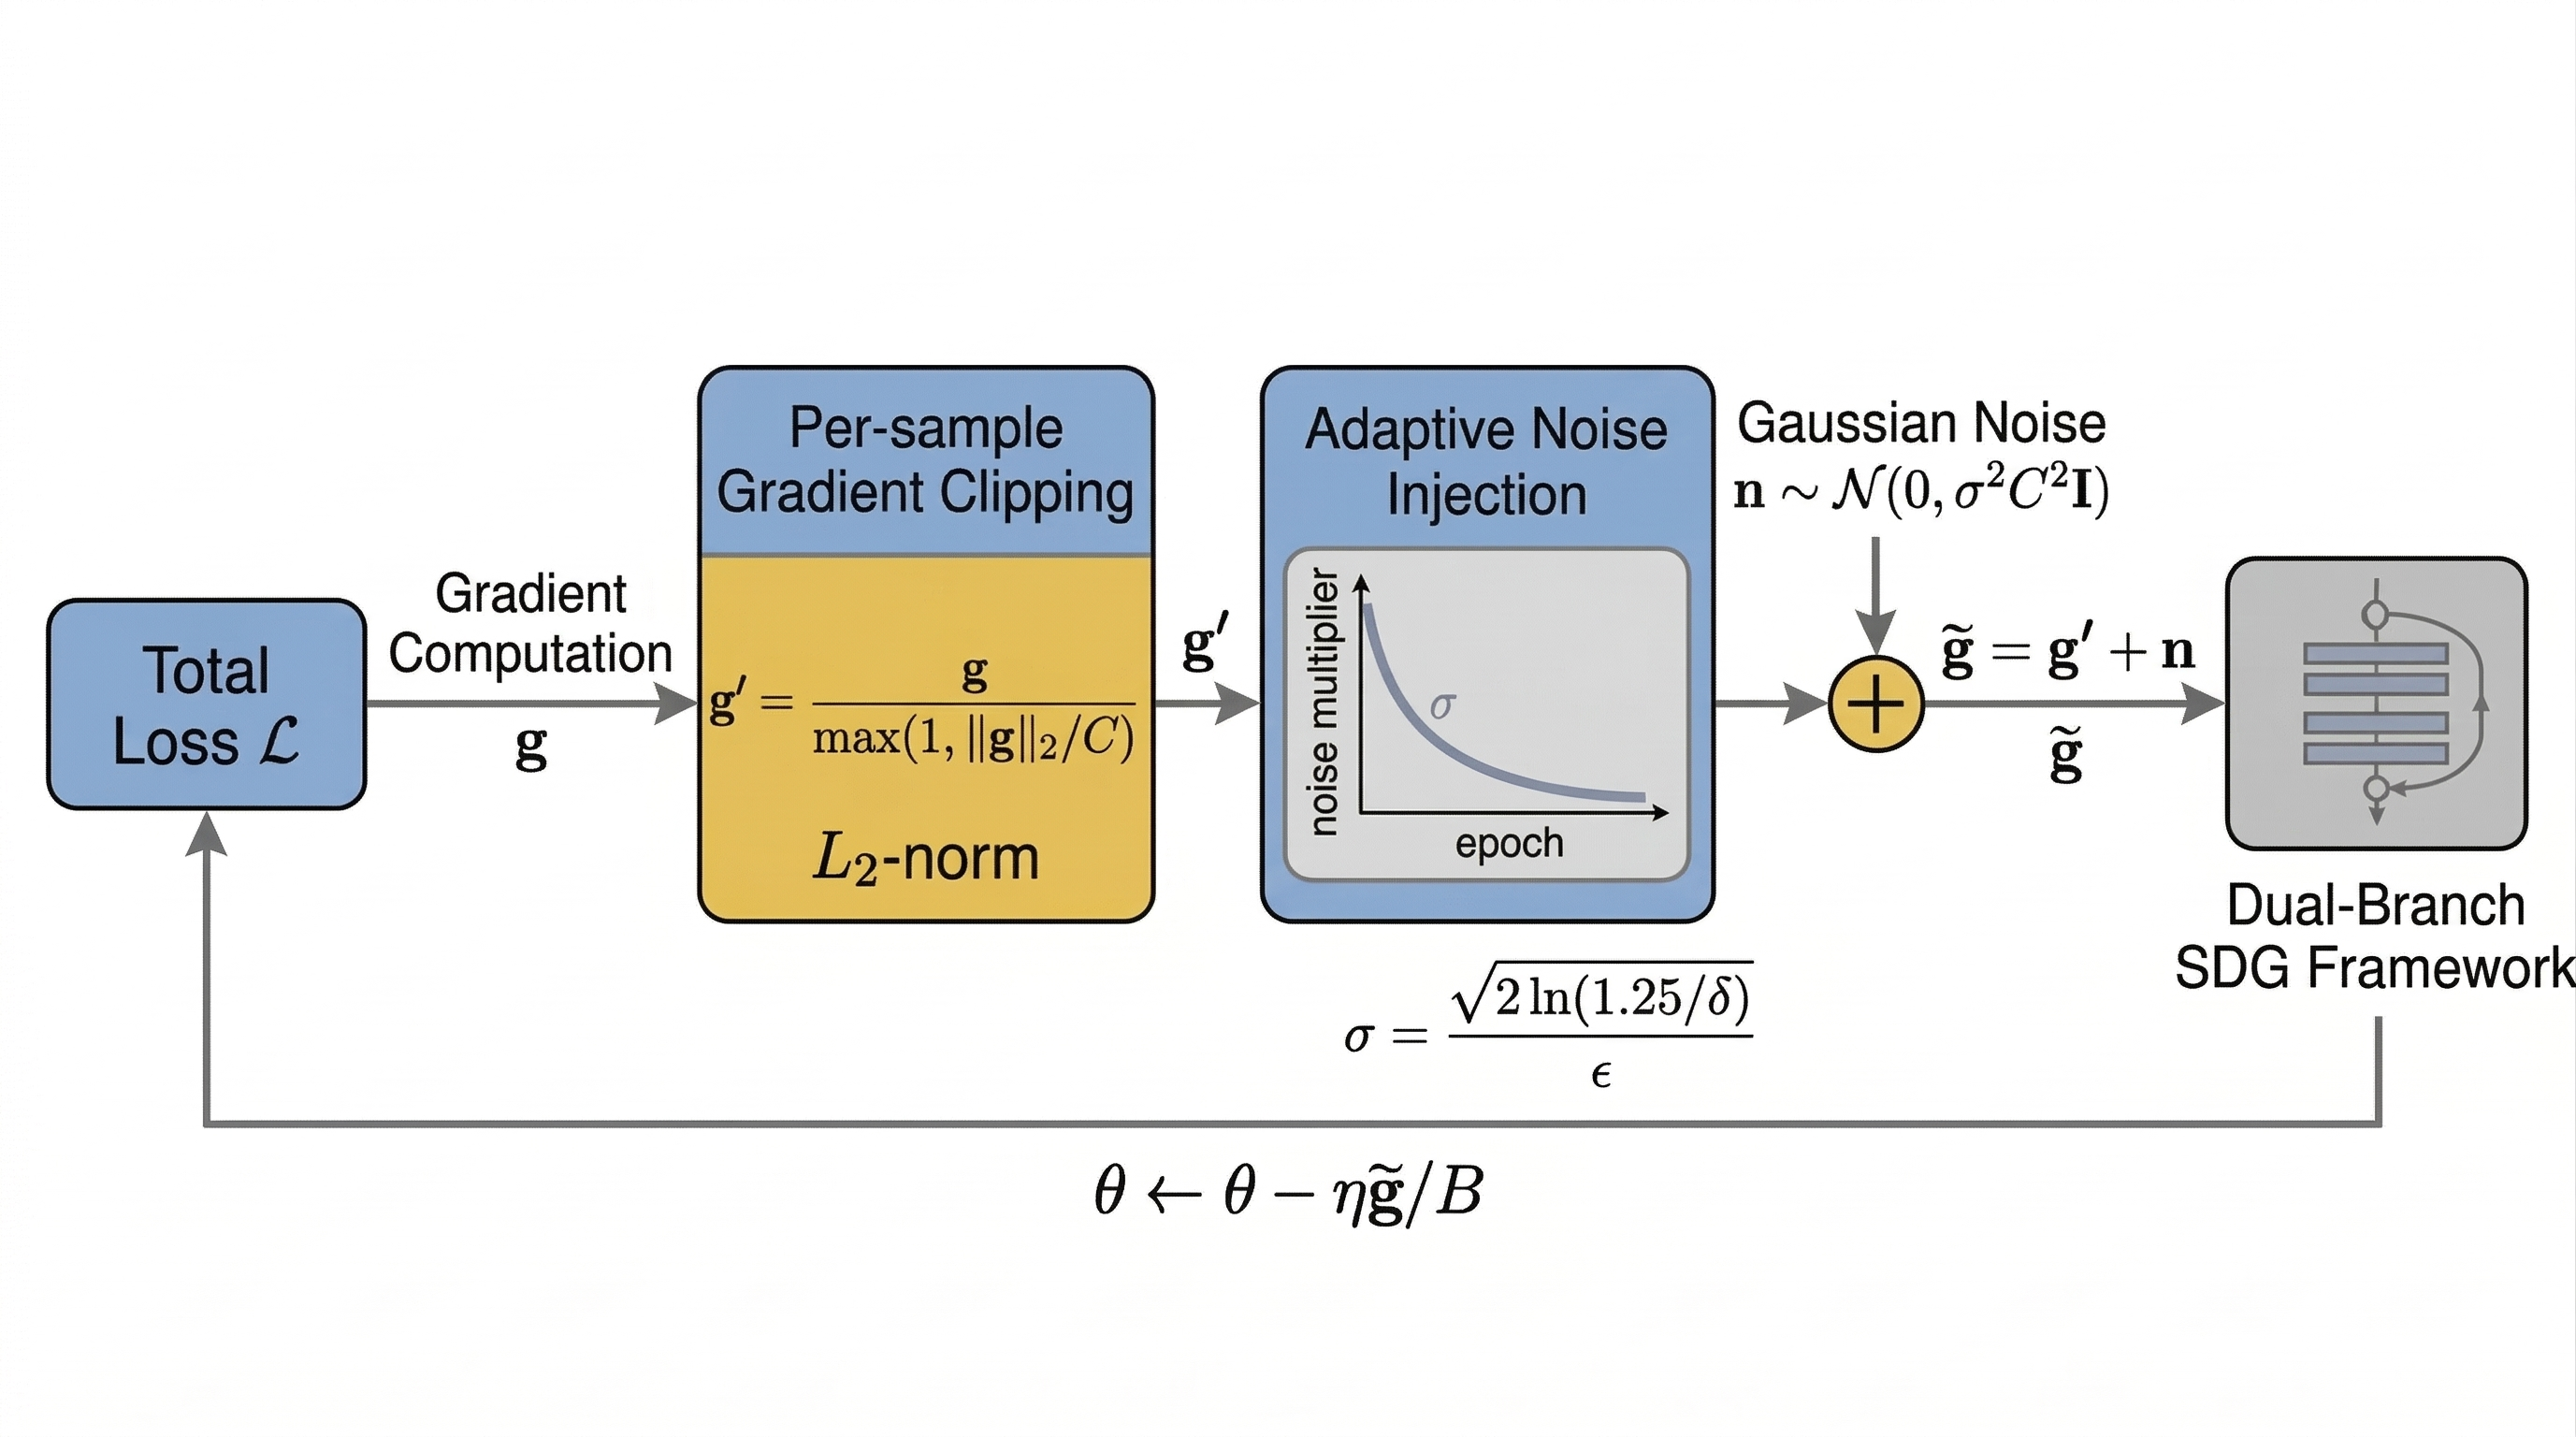
\includegraphics[width=0.82\textwidth]{images/media/image3_v2.png}
\caption{Integration of Adaptive Gaussian Differential Privacy into the single-domain generalization framework. During training, each update first clips per-sample gradients, then injects Gaussian noise and updates the parameters. Unlike fixed-noise differential privacy, this study adopts a noise multiplier that is adaptively adjusted and gradually decayed with the training stage.}
\label{fig:privacy-framework}
\end{figure}

\revision{Differential privacy characterizes the influence of an individual training example on the output distribution of a randomized algorithm. The privacy definition in this study is formulated at the example level, where each example consists of a fundus image and its associated multi-label annotation. Two datasets $D$ and $D'$ are adjacent when they differ in one training example. A randomized algorithm $M$ satisfies $(\epsilon,\delta)$-DP if, for every pair of adjacent datasets and every measurable output set $S$,}

\begin{equation}\label{eq:dp-definition}
\Pr\lbrack M(D) \in S\rbrack \leq e^{\epsilon}\Pr\lbrack M(D') \in S\rbrack + \delta,
\end{equation}

\revision{Here, $\epsilon$ controls the multiplicative bound on output probabilities, while $\delta$ is the additive relaxation term. Under the same adjacency definition and $\delta$, a smaller $\epsilon$ specifies a tighter privacy constraint. The privacy experiments in this study use $\delta=10^{-5}$ and report cumulative $\epsilon$ values alongside recognition performance.} Under the DP-SGD framework, the per-sample gradient \(g\) is first clipped by its L2 norm at each iteration:

\begin{equation}\label{eq:gradient-clip}
g' = g/max(1, \parallel g \parallel_{2}/C),
\end{equation}

Gaussian noise \(n \sim \mathcal{N}(0,\sigma^{2}C^{2}I)\) is then added, where \(\sigma\) is the noise multiplier controlling noise intensity. It is usually related to the privacy budget \(\epsilon\) and relaxation parameter \(\delta\), and can be written as:

\begin{equation}\label{eq:noise-multiplier}
\sigma = \sqrt{2\ln(1.25/\delta)}/\epsilon.
\end{equation}

The noisy gradient is \(\widetilde{g} = g' + n\), and the parameters are updated as \(\theta \leftarrow \theta - \eta\widetilde{g}/B\), where \(B\) is the batch size. \revision{Differential privacy relates the noise required for information protection to the sensitivity of the released quantity \mbox{\cite{_Ref214903493}}. For neural-network training, Abadi et al. \mbox{\cite{_RefAbadi2016DP}} combine per-example gradient clipping, Gaussian noise added to aggregated gradients, and privacy accounting across repeated updates. This construction bounds the influence of individual training examples and quantifies the cumulative privacy loss of training.}

\revision{For mechanisms satisfying R\'enyi differential privacy, Balle et al. \mbox{\cite{_RefBalle2022Reconstruction}} derive an upper bound on reconstruction success given a prior over the target sample, a reconstruction error measure, and a specified accuracy threshold. Their analysis links the privacy parameters of a training mechanism to the risk of reconstructing an individual training sample. Together, these studies provide a theoretical basis for incorporating gradient perturbation into the proposed single-source framework to address leakage of source-domain training information.}

\revision{However, when a fixed noise multiplier is used throughout training, noise perturbations in the later stages may still affect model convergence and final recognition performance. To address this issue, this study adopts an Adaptive Gaussian Differential Privacy (AdaGDP) mechanism in training the joint DFE--ARC model. A larger noise multiplier is used early in training for source-domain training-information protection, and the noise intensity is then gradually reduced according to a predefined decay rate to limit its impact on later-stage optimization. The learning rate and its schedule are configured in conjunction with the noise schedule to support disease-discriminative learning under gradient perturbation. During training, cumulative $\epsilon$ values and recognition performance are recorded at different epochs to examine recognition utility as the reported privacy budget increases. The results in Section~4.5 show that this training configuration retains recognition performance close to the official non-private ODIR ResNet50 baseline, illustrating the trade-off between training-information protection and recognition utility.}
